\chapter{Analýza}
% popis Manty
\section{Manta Flow}
\textit{Manta Flow}\footnote{https://getmanta.com/} je nástroj umožňující automatickou analýzu zdrojového kódu (\textit{SQL}, Java) a následný popis transformační logiky v něm obsažené. Software je schopný rozpoznat i těžce čitelné konstruky zdrojového kódu. Díky tomu dokáže automaticky zanalyzovat rozsáhlé databáze a vytvořit z nich přehlednou mapu datových toků, neboli \textit{Data Lineage}. To se v praxi využívá převážně k optimalizaci datových skladů, snižování nákladů na vývoj softwaru, provádění dopadových analýz a při dokumentování prostředí pro potřeby regulačních úřadů.

V souladu s architektonickým stylem \textit{klient - server} má aplikace dvě hlavní komponenty (viz diagram \ref{fig:ana-flow-comp}):
\begin{itemize}
	\item{\textit{Manta Flow CLI}}: je Java řádková aplikace provádějící extrakci skriptů ze zdrojových databází a uložišť a jejich analýzu. Analyzovaná data jsou následně poslána \textit{Manta Flow Serveru}. \textit{Klientská aplikace} také může nahrávat vygenerované exporty ze \textit{serveru} do externí metadatové databáze.
	\item{\textit{Manta Flow Server}}: je serverová Java aplikace, která ukládá získané informace do interního metadatového uložiště, transformuje je, umožňuje jejich visualizaci a přístup k nim pomocí veřejného \textit{API}.
\end{itemize}

Interakce mezi \textit{klientskou} a \textit{serverovou} částí aplikace je popsána zjednodušeným sekvenčním diagramem \ref{fig:ana-flow-seq}. Tento proces je označován jako \textit{merge} a je blíže popsán v kapitole \ref{sec:ana_merger}.
Pro tuto práci je podstatná především \textit{serverová} část aplikace a její interakce s metadatovým uložištěm (kapitola \ref{sec:ana_components}). \textit{Klientská} část aplikace je proto popsána méně detailně (kapitola \ref{sec:ana_other}).


\section{Metadatové uložiště}
\label{sec:ana_model}
Jak již bylo zmíněno v úvodu práce (kapitola \ref{sec:uvod}) metadatové uložiště produktu \textit{Manta Flow} je aktuálně implementováno grafovou databází \textit{Titan} (ve verzi 0.4) a je snaha o výměnu této databáze\cite{Kovar18}.
Než přistoupíme k bližšímu popisu jednotlivých komponent aplikace a jejich interakcí s metadatovým uložištěm (kapitola \ref{sec:ana_components}, je třeba nejdříve popsat entity, které jsou součástí analýzy datových toků a datový model metadatového uložiště (zobrazený na obrázku \ref{fig:ana-model}\footnote{Z modelu metadatového uložiště je zřejmé, že ne všechny podgrafy tvoří \textit{strom}. Vlastnosti \textit{stromu} nicméně porušují pouze hrany typu \textit{directFlow} a \textit{filterFlow}, které jsou výsledkem analýzy datových toků a jejichž odstraněním by strom vznikl. V textu je tak v některých případech používána teminologie vztahující se ke \textit{stromům} (například \textit{kořen}) - na celý graf je nahlíženo jako ne \textit{les}.}).

% entity datového modelu
V procesu analýzy datových toků hraje roli mnoho entit z analyzovaných systémů. Ty se navíc mohou výrazně lišit systém od systému - \textit{Manta Flow} může analyzovat širokou škálu spolu propojených databázových systémů a integračních služeb. Obecně lze říci, že každý systém obsahuje zdroje a cíle dat (tabulky, soubory, ...) a transformace dat (skripty, \textit{\nomExpl{ETL}{Extract Load Transform}} workflow, procedury, makra a další).

\begin{figure}
\begin{center}
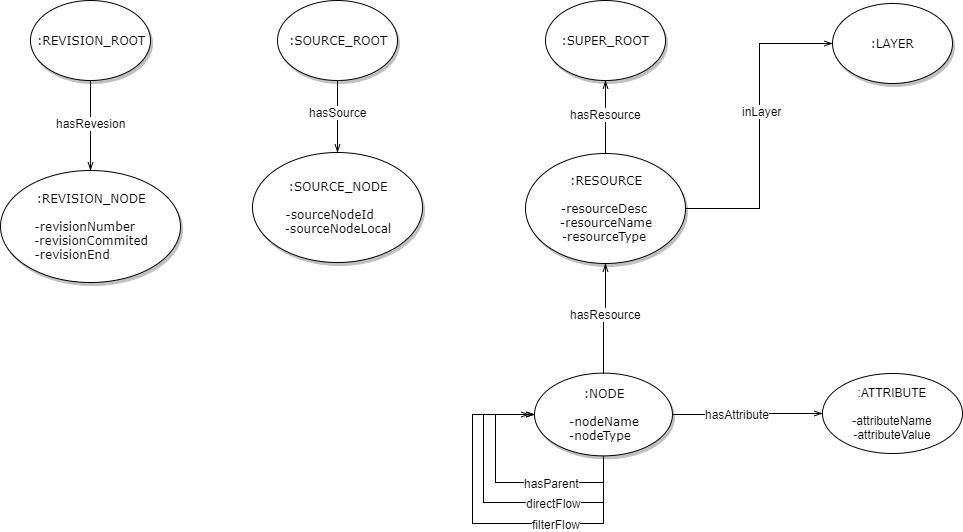
\includegraphics[width=14cm]{figures/model}
\caption{Model grafové databáze}
\label{fig:ana-model}
\end{center}
\end{figure}

% datový model
Samotný datový model se skládá z devíti typů uzlů:

\begin{itemize}
	\item{\textit{SUPER\_ROOT}}: Uzel (právě jeden v databázi), který slouží jako umělý kořen všech uzlů typu \textit{RESOURCE}.
	\item{\textit{RESOURCE}}: Uzly tohoto typu reprezentují zdrojové systémy - zdroje definic objektů, zdrojových kódů, \textit{ETL} řešení a další.
	\item{\textit{NODE}}: Uzly typu \textit{NODE} představují reálné objekty zdrojového systému - databáze, tabulky, sloupce, procedury, skripty a další.
	\item{\textit{LAYER}}: Uzly typu \textit{LAYER} reprezentují vrstvy modelu metadat. Datové toky nalezené při analýze zdrojových kódů jsou vždy ukládány do \textit{fyzické vrstvy}, ze které je potom možné generovat abstraktnější vrstvy modelu datových toků.
	\item{\textit{ATTRIBUTE}}: Uzly typu \textit{ATTRIBUTE} reprezentují atributy uzlů typu \textit{NODE} - parametry sloupců, popisy databázových objektů a další.
	\item{\textit{SOURCE\_ROOT}}: Uzel (právě jeden v databázi), který slouží jako umělý kořen všech uzlů typu \textit{SOURCE\_NODE}.
	\item{\textit{SOURCE\_NODE}}: Uzly typu \textit{SOURCE\_NODE} reprezentují soubory se zdrojovými kódy extrahovanými ze zdrojových systémů.
	\item{\textit{REVISION\_ROOT}}: Uzel (právě jeden v databázi), který slouží jako umělý kořen všech uzlů typu \textit{REVISION\_NODE}.
	\item{\textit{REVISION\_NODE}}: Uzly typu \textit{ATTRIBUTE} reprezentují revize modelu metadat, definují tedy jeho verzování. Kromě dalších parametrů mají všechny hrany grafu parametry \textit{tranEnd} a \textit{tranStart} definující platnost hran (viz obrázek \ref{fig:ana-model-rev}). Při každé analýze zdrojových systémů (která je prováděna dávkově klientskou částí aplikace) je vytvořena nová revize metadatového uložiště obsahující všechny objekty zdrojových systémů.\footnote{Je snaha tento princip upravit tak, aby byly objekty v metadatovém uložišti minimálně repklikovány \cite{Sykora17}.}
\end{itemize}

 a osmi typů hran:

 \begin{itemize}
	\item{\textit{hasResource}}: Hrana přiřazuje objekty (uzly typu \textit{NODE}) ke svým zdrojovým systémům (uzlům typu \textit{RESOURCE}). Hrana je také použite k propojení uzlů typu \textit{RESOURCE} s uzlem \textit{RESOURCE\_ROOT}.
	\item{\textit{hasParent}}: Hrana mezi dvěmi uzly typu \textit{NODE} vytvářející klasickou hiearchickou strukturu mezi těmito uzly - strom závislostí objektů zdrojových systémů.
	\item{\textit{directFlow}}: Hrana mezi dvěmi uzly typu \textit{NODE} říkající, že mezi těmito uzly existuje přímý datový tok (ve směru hrany).
	\item{\textit{filterFlow}}: Hrana mezi dvěmi uzly typu \textit{NODE} říkající, že mezi těmito uzly existuje nepřímý datový tok (ve směru hrany).
	\item{\textit{hasAttribute}}: Hrana přiřazující uzlům typu \textit{NODE} jejich atributy (uzly typu \textit{ATTRIBUTE}).
	\item{\textit{inLayer}}: Hrana typu \textit{inLayer} spojeju zdroje (uzly typu \textit{RESOURCE}) a vrstvy a říká, že zdroj patří do dané vrstvy modelu metadat.
	\item{\textit{hasSource}}: Hrana je použita k propojení uzlů reprezentujících zdrojové kódy (uzly typu \textit{SOURCE\_NODE}) s uzlem \textit{SOURCE\_ROOT}.
	\item{\textit{hasRevision}}: Hrana je použita k propojení uzlů reprezentujících revize modelu metadat (uzly typu \textit{REVISION\_NODE}) s uzlem \textit{REVISION\_ROOT}.
\end{itemize}

\begin{figure}
\begin{center}
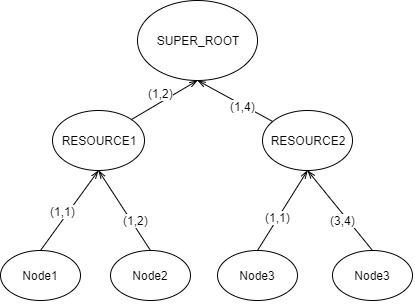
\includegraphics[width=6cm]{figures/model_revisions}
\caption{Způsob verzování modelu metadat}
\label{fig:ana-model-rev}
\end{center}
\end{figure}

Uzly i hrany mají dle svého typu několik specifických atributů, ty ale nebudeme blíže popisovat, protože nejsou pro analýzu zásadní.

V metadatovém uložišti je dále definováno několik typů indexů, konkrétně se jedná o standardní indexy:

\begin{itemize}
	\item{\textit{indexy na kořeny}}: indexy pro konkrétní uzly, kořeny jednotlivých stromů datového modelu - \textit{SUPER\_ROOT, SOURCE\_ROOT, REVISION\_ROOT}
	\item{\textit{indexy na atributy hran}}: indexy zrychlující dohledávání atributů hran
	\item{\textit{indexy na typy hran}}: indexy zrychlující dohledávání hran daného typu pro jednotlivé uzly
\end{itemize}

a externí \textit{Apache Lucene} indexy, které slouží pro \textit{fulltextové} vyhledávání uzlů dle jejich názvů a pro intervalové vyhledání revizí.


\section{Popis komponent serverové části}
\label{sec:ana_components}

Aplikace \textit{Manta Flow} praceje s metadatovým uložištěm několika různými způsoby, přičemž různé moduly aplikace využívají jeden či více těchto přístupů (a často také provádí vlastní pomocné dotazy přímo do metadatového uložiště). Cílem této sekce je tyto způsoby manipulace s metadatovým uložištěm identifikovat a popsat (není tedy účelem detailní technický popis všech dotazů do metadatového uložiště, ale spíše popis obecných principů a specifických situací - například netradiční zacházení s transakcemi).

\subsection{Connector}
\label{sec:ana_connector}
Modul, který je nejblíže metadatovému uložišti, tzv. \textbf{connector} má dvě hlavní zodpovědnosti - zajištění připojení aplikace k uložišti a provádění dotazů nad ním.

%Operations
Modul obsahuje sadu základních dotazů, tzv. \textit{operatinos}, mezi které patří například:
\begin{itemize}
	\item{získání předka uzlu}
	\item{získání atributů uzlu}
	\item{získání sousedních uzlů a hran}
	\item{získání cesty ke kořeni}
	\item{získání podstromu}
\end{itemize}
Tyto operace přímo přistupují do databáze a pomocí programovacího jazyka \textit{Gremlin}\footnote{Používá se \textit{TinkerPop} ve verzi \textit{2.6}.} a jsou na nich postaveny složitější operace nad grafouvou databází. U základních operací nejsou transakce řízeny explicitně, ale implicitně grafovou databází.

% Algorithm
Další částí modulu \textit{connector} jsou tzv. algoritmy, tedy komponenta, pomocí které jsou v metadatovém uložišti hledány samotné datové toky. Tato komponenta řetězí několik grafových algoritmů, přičemž první z nich získá z metadatového uložiště podmnožinu datových toků, která je dalšími algoritmy filtrována a omezována. Tímto způsobem vzniká tzv. \textit{referenční view} - objekt obsahující kompletní graf datových toků pro zadané výchozí uzly a směr datových toků. To je pak využ   íváno dalšími moduly aplikace, například \textit{viewerem} (viz \ref{sec:ana_viewer}), který dle parametrů zadaných ve webové aplikaci graf datových toků vizualizuje.
Jednotlivé algoritmy používají výše popsané základní operace (\textit{operations}) a v některých případech také samy dotazují metadatové uložiště přímo pomocí jazyka \textit{Gremlin}.

% Traversal
Posledním způsobem manipulace s metadatovým uložištěm, který modul umožňuje je přístup pomocí \textit{traversalů}. Ty pracují na obecném principu \textit{traversování} grafů popsaném v kapitole \ref{sec:gdb-dotazy}. V tomto případě ale celý průchod grafem není realizován samotnou grafovou databází, ale přímo aplikací, přičemž grafová databáze je dotazována pouze na dílčí informace - například na okolní uzly. \textit{Traversaly} jsou používány v případech, kdy je manipulováno s větší částí grafové databáze, například při jejím exportu. Tyto operace jsou realizovány \textit{vizitory} - každý uzel, který je procházen \textit{traversalem} je následně obsloužen \textit{vizitorem}, který provede požadovanou operaci (jedná se o návrhový vzor \textit{Visitor} - viz \cite{Gamma94}). Obě tyto části, tedy procházení grafu \textit{traversalem} i obsloužení všech objektů \textit{visitorem} jsou prováděny za pomocí základních grafových operací definovaných výše (\textit{operations}). Zároveň je ale také z tohoto kontextu grafová databáze dotazována přímo pomocí jazyka \textit{Gremlin}. Jedná se ale spíše o jednoduché dotazy na dohledání uzlů, jejich atributů apod.

\subsection{Merger}
\label{sec:ana_merger}
\textit{Merger} je modul, který je používán při analýze zdrojových systémů. Slouží k zanesení výsledků dílčích analýz jednotlivých částí (např. skriptů) zdrojových systémů do metadatového uložiště.

Vlastní operace \textit{merge}\footnote{Operace \textit{merge} má v kontextu aplikace \textit{Manta Flow} obdobný význam, jako například v \textit{SQL}: pokud objekt není uložen v persistentní vrstvě, je do ní uložen (\textit{insert}), jinak je aktualizován (\textit{update}).} lze zjednodušeně popsat pseudokódem \ref{alg_merger} (správa transakcí a synchronizace je blíže popsána v kapitole \ref{sec:ana_transactions}). Ten je uveden především kvůli složitému transakčnímu modelu, jehož účelem je umožňení provádění dotazů do metadatového uložiště jinými částmi aplikace, zatímco je prováděn \textit{merge} analyzoných částí zdrojových systémů.

Operace se chová různě v případě, kdy je umožňěno verzovaní metadatového uložiště (a to tak obsahuje více revízí) a kdy je vypnuto. V případě zapnutého verzování je \textit{merge} prováděn vždy do nové revize, pokud je verzování vypnuté, je prováděn do hlavní (jediné) revize.

Samotné \textit{merge} operace nad objekty grafové databáze (uzly, hranami, atributy, ...) jsou prováděny přímímy dotazy do databáze pomocí jazyka \textit{Gremlin}. K přístupu do metadadtového uložiště se tedy nevyužívá modul k tomu předurčený - \textit{Connector} (viz \ref{sec:ana_connector}).

\begin{algorithm}
\caption{Merger pseudocode}
\label{alg_merger}
\begin{algorithmic}
	\State $acquireGraphLock()$
	\State $revision\gets getNewestRevision()$
	\If {$revision.isOpen()$}
		\State $acquireScriptsLock()$
		\ForAll{$script in scripts$}
			\State $beginWriteTransaction()$
			\State $merge(script)$
			\State $conditionalCommit()$
		\EndFor
		\State $releaseScriptsLock()$
		\State $beginWriteTransaction()$
		\ForAll{$object in objects$}
			\State $merge(object)$
			\State $periodicalCommit()$
		\EndFor
	\EndIf
	\State $releaseGraphLock()$
\end{algorithmic}
\end{algorithm}

\subsection{Viewer}
\label{sec:ana_viewer}
\textit{Viewer} je modul sloužící k poskytování dat uživatelskému rozhraní aplikace (klientské části webové aplikace). Jeho nejčastější interakce s metadatovým uložištěm je dotaz na \textit{referenční view} dle parametrů zadaných uživatelem. To je prováděno pomocí algoritmů definovaných v modulu \textit{connector} (viz \ref{sec:ana_connector}), který obsahuje algoritmy pro hledání datových toků (resp. \textit{referenčního view}).

Kromě toho \textit{viewer} dotazuje metadatové uložiště o další informace, které následně propaguje do uživatelského rozhraní - především o informace o revizích metadatového uložiště a o objekty zdrojových systémů, pomocí kterých uživatel vybírá výchozí uzly pro hledání datových toků (\textit{referenčního view}). Informace o revizích metadatového uložiště jsou dohledávány pomocí základních operací definovaných v modulu \textit{connector} (viz \ref{sec:ana_connector}) a pomocí přímých dotazů do metadatového uložiště pomocí jazyka \textit{Gremlin} s explicitního řízení transakcí. Pro vyhledávání objektů zdrojových systémů (v metadatovém uložišti uzly typu \textit{NODE}, viz \ref{sec:ana_model}) je použito vyhledávání pomocí fulltextového indexu implementovaného pomocí \textit{Apache Lucene}. Ten indexuje uzly v metadatovém uložišti podle jejich názvu a umožňuje jejich rychlé vyhledávání.


\subsection{Public API}
\label{sec:ana_public}
\textit{Public API} je modul, který by měl umožňovat vzdálené volání veřejné části funkcionality aplikace pomocí \textit{REST API}. Konkrétně lze tímto způsobem volat například analýzu datových toků mezi různými objekty zdrojového systému. Modul přepoužívá část funkcionality poskytovanou modulem \textit{connector}, část těchto funkcionalit ale duplikuje (s menšími úpravami) a přímo tak dotazuje metadatové uložiště.

\subsection{Exporter}
\label{sec:ana_exporter}
Posledním modulem, který přímo interaguje s metadatovým uložištěm je \textit{exporter}, jehož úkolem je exportovat aktuální stav grafové databáze (ne nutně vše, může být exportován například jen interval revizí atd.) buďto do \textit{CSV} souborů, nebo přímo do formátu používaného dalšími nástroji používanými na správu metadat. \textit{Exporter} jako nástroj pro práci s metadatovým uložištěm nejčastěji používá \textit{traversery} a \textit{observery} poskytované modulem \textit{connector}, díky kterým je možné provádět operace nad velkou částí metadatového uložiště bez zásadních paměťových požadavků. Dále jsou využívány základní základní operace (\textit{operations}) poskytované stejným modulem a v některých případech je metadatové uložiště dotazováno přímo pomocí jazyka \textit{Gremlin}.


\section{Popis ostatních komponent}
\label{sec:ana_other}
\subsection{Manta Flow CLI}
Klientská část aplikace \textit{Manta Flow} je \textit{command line} aplikace implementovaná v programovacím jazyce Java sestavená z několika modulů. Jejím hlavním úkolem je extrakce skriptů ze zdrojových databázových systémů a repozitářů (modul \textit{Exktractor}), a jejich následné parsování a analýza (modul \textit{Analyzer}). Analýza skriptů probíhá v klientské části aplikace z toho důvodu, že využívá vyextrahované slovníky objektů zdrojového systému, které by v případě provádění analýzy serverovou částí aplikace musely být přenášena na server spolu se skripty. Poté, co proběhne zpracování (\textit{merge} - viz. kapitola \ref{sec:ana_merger}) zanalyzovaných skriptů serverem, výsledky jsou vyexportovány zpět do klientské části aplikace, odkud mohou být případně nahrány do externí metadatové databáze.

\subsection{Configurator}
\label{sec:ana_configurator}
\textit{Configurator} je \textit{standalone} webová aplikace implementovaná v programovacím jazyce Java (jako třívrstvá aplikace), jejímž úkolem je poskytnout \textit{grafické uživatelské rozhraní (GUI)}, pomocí kterého může uživatel změnit komplexní konfiguraci aplikace \textit{Manta Flow}. Konfigurace je typicky obsažena v \textit{properties} souborech a to na různých místech. Serverová a klientská část \textit{Manta Flow} má vlastní konfiguraci. \cite{Molitor18}

\subsection{Updater}
\label{sec:ana_updater}
\textit{Updater} je \textit{standalone} webová aplikace implementovaná v programovacím jazyce Java (jako třívrstvá aplikace), jejímž úkolem je poskytnout \textit{GUI}, které provede uživatelem \textit{updatem} aplikace \textit{Manta Flow} (konkrétně její serverové části) na novější verzi. Aplikace umožňuje uživateli provést změny v komplexní konfiguraci aplikace a provede \textit{merge} těchto změn s původním nastavením. \cite{Gondek16}

\section{Požadavky a omezení}
\label{sec:ana_problems}
V následujících podkapitolách jsou popsány aktuální architektonická omezení a problémy aplikace \textit{Manta Flow}. Cílem nově navržené architektury je, aby řešila problémy pramenící z nevhodné manipulace s grafovou databází představující metadatové uložiště a umožnila řešení ostatních problémů popsaných v této kapitole.

\subsection{Datová konzistence}
\label{sec:ana_transactions}
Z popisu jednotlivých komponent aplikace v kapitolách \ref{sec:ana_components} a \ref{sec:ana_other} je patrné, že je používáno několik heterogenních přístupů k manipulaci s daty (především v grafové databázi) a je tak třeba pečlivě řídit konzistenci dat. Primárním princepem zaručujícím konzistenci dat je verzování modelů datových toků na jednotlivé \textit{major} a \textit{minor} revize \cite{Sykora17}.
Cílem je, aby všechny moduly, které pouze provádějí analýzu datových toků a tu předávají (v některé z dostupných forem) dále, tedy \textit{Viewer}, \textit{Exporter} a \textit{Public API}\footnote{Pomocí \textit{Public API} může být grafová databáze i upravována, všechny úpravy jsou ale prováděny pouze pomocí modulu \textit{Merger}.} mohly být spouštěny nad některou z uzavřených (\textit{commitnutých}) revizí, zatímco \textit{Merger}, který vkládá nové informace na základě analýzy provedené klientskou částí aplikace, má k dispozici jednu otevřenou \textit{necommitnutou} pracovní revizi. Všechny zmíněné moduly používají pro přístup do grafové databáze primárně modul \textit{Connector}, který obsahuje operace čtení i zápisu, obecně ale platí, že operace zápisu jsou používány pouze \textit{Mergerem}.
I přes systém revizí může vzniknout často konkurence při čtení a zápisu dat do grafové databáze:

\begin{itemize}
	\item{\textit{Úprava uzavřené revize}}: Při vytváření nové revize, která vzniká typicky jako \textit{full update} celého modelu datových toků\footnote{Nová \textit{major} revize vzniká jako \textit{full update} modelu datavých toků, nová \textit{minor} revize jako \textit{incremental update}. Konkrétní implementace obou operací se v některých detailech liší, z pohledu datové konzistence ale řeší oba přístupy koncepčně stejný problém. Můžeme proto analýzu vzniku nové revize datového modelu zobecnit na \textit{full update} přístup - tedy na \textit{major} revize.}, může nastat několik situací. Připomeňme, že platnost vztahu mezi dvěmi uzly je parametrem hrany spojující tyto uzly. Pokud se libovolné dva uzly a jejich vztah nezmění mezi uzavřenou revizí \textit{A} a vznikající neuzavřenou revizí \textit{B}, pak jsou upraveny atributy hrany reprezentující tento vztah a může tak vzniknout konkurence při čtení revize \textit{A} a zápisu do revize \textit{B}.
	\item{\textit{Kombinace operací pro čtení a zápis při vytváření nové revize}}: Modul \textit{Merger} při vytváření nové revize modelu datových toků v grafové databází spouští několik komplexních postproccessingových algoritmů, které vyžadují přístup pro čtení i zápis do pracovní otevřené revize (a jsou v některých případech prováděny paralelně).
	\item{\textit{"Stop the world" operace}}: Je také definováno několik takzvaně "stop the world" operací, tedy operací, při kterých je znepřístupněna velká část, nebo přímo celá grafová databáze. Mezi tyto operace patří odstraňování starých revizí modelu datových toků, import či export kompletního \textit{dumpu} grafové databáze.
\end{itemize}

Vzhledem k výše uvedeným situacím je konkurence při přístupu k datům řízena dvěmi dalšími mechanikami, kterými jsou databázové transakce a synchronizace pomocí \textit{reentrant} zámků.

Transakce jsou řízeny programaticky\footnote{Kromě programatického řízení transakcí je možné použít i deklarativní řízení transakcí (\textit{Declarative Transaction Model}). Ne pro všechny grafové databáze ale v tuto chvíli existují implementace, které by deklarativní transakce v rámci \textit{Spring} frameworku umožňovaly. V tuto chvíli je podporuje například \textit{Orient DB} (\url{https://github.com/orientechnologies/spring-data-orientdb}) a databáze přístupné pomocí \textit{TinkerPop Gremlin 2.x} (\url{https://github.com/gjrwebber/spring-data-gremlin}). Podpora pro \textit{Apache TinkerPop 3.x} je aktuálně ve vývoji.} (\textit{Programatic Transaction Model} \cite{Little04}) za pomoci implementace \textit{Spring TransactionTemplate}\footnote{\url{https://docs.spring.io/spring/docs/current/javadoc-api/org/springframework/transaction/support/TransactionTemplate.html}} kombinující \textit{Titan} transakce a Java \textit{reentrant} zámky.
\textit{Titan} v případě transakcí pouze přeposkytuje funkcionalitu používané podkladové databáze, kterou je v případě \textit{Manta Flow} embedded NoSQL databáze typu klíč-hodnota \textit{Persistit}\footnote{\url{https://github.com/pbeaman/persistit}}. Ta, stejně jako mnoho dalších grafových databází, implementuje \textit{Multi-Version Concurrency Control (MVCC)} \cite{Prakash10} využívající \textit{Snapshot Isolation}\footnote{Všechny záznamy v databázi jsou verzovány. Při čtení transakce vytvoří kopii poslední \textit{commitnuté} verze čteného záznamu, ta je po ukončení transakce odstraněna. \textit{Snapshot isolation} tak v zásadě odpovídá úrovni izolace transakcí \textit{Read committed}.} úroveň izolace transakcí.
Jedná se o \textit{optimistický} transakční model, žádné databázové objekty (ani záznamy) nejsou zamykány, takže transakce probíhají v plné rychlosti bez čekání. Může tak ale nastat situace, že ne všechny transakce je možné \textit{commitnout} a jedna (nebo více) z těchto transakcí tak musí být zrušena (a zopakována). \textit{Snapshot} izolace transakcí má v grafových databázích také další specifický důsled. Zatímco v případě relačních databází vždy existuje unikátní identifikátor každého záznamu (byť i implicitní), v grafových databázích tomu tak není - tedy neexistuje žádná unikátnost uzlů a hran v grafové databázi za předpokladu, že není explicitně vynucena pomocí unikátních indexů. Ty nejsou v aplikaci \textit{Manta Flow} používány, může tak nastat situace, kdy se dvě transakce souběžně snaží o vytvoření (z pohledu aplikační logiky) identického uzlu či hrany, obě transakce uspějí (nedojde k jejich kolizi) a objekt je tak vytvořen dvakrát (čímž je zanesena nekonzistence do metadatového uložiště).
Aby k těmto konfliktům paralelních transakcí nedocházelo, používá aplikace při přidělování transakcí synchronizaci pomocí \textit{reentrant} zámků, přičemž vlastní zámek je pro obecné transakce a vlastní pro \textit{read-only} transakce. Nemohou tak současně existovat dvě transakce, které by mohly do databáze zapisovat zároveň - což může potenciálně velmi snižovat rychlost prováděných operací. Důsledkem tohoto systému zámků je serializace paralelních klientských požadavků pro zápis do metadatového uložiště (\textit{merge}). Tento process v klientské části aplikace přitom probíhá paralelně, tipicky minimálně ve čtyřech vláknech.

Další používanou synchronizační mechanikou je zamykání grafové databáze (respektive uzlů reprezentující jednotlivé revize) \textit{reentrant read-write} zámkem při několika operacích, které jsou součástí \textit{Mergeru} a importu a exportu \textit{dumpu} grafové databáze. Tyto zámky tak společně s verzováním modelu metadat slouží při \textit{mergi} de-facto jako implementace \textit{long living} transakcí - samotný \textit{merge} objektů do grafové databáze je prováděn v několika transakcích\footnote{Transakce jsou objektem uloženým v operační paměti, přičemž velikost transakce narůstá s počtem úprav v databázi.}.

Poslední synchronizace na straně serveru je zamykání metadatové databáze nesoucí informace a zanalyzovaných skriptech pro účely kontroly licencí. K této synchronizaci dochází při \textit{mergi} v okamžiku, kdy jsou informace o skriptech do metadatového uložiště nahrávány.


\subsection{Výkon aplikace}
\label{sec:ana_performance}
Výkon je významným kvalitativním kritériem aplikace. U různých procesů jsou přitom požadavky na výkon různé:
\begin{itemize}
	\item{\textit{Analýza datových toků}}: Analýza datových toků probíhá v reálném čase na základě požadavku uživatele (pomocí \textit{GUI} aplikace poskytované modulem \textit{Viewer} - kapitola \ref{sec:ana_viewer}), nebo pomocí \textit{REST API} - kapitola \ref{sec:ana_public}). Maximální \textit{response time} požadavku je tedy v řádu jednotek vteřin. Toho je docíleno především optimalizací algoritmů počítajících datové toky na základě uživatelského požadavku a optimalizací dotazování metadatového uložiště pomocí interních a externích indexů (kapitola \ref{sec:ana_model}).

	\item{\textit{Update metadatového uložiště}}: Narozdíl od výpočtu datových toků je update metadatového uložiště dávkový (typicky noční) proces, který probíhá v závislosti na procesech uživatelů \textit{Manta Flow} jednou denně až jednou měsíčně\footnote{Předpokládá se, že v návaznosti na zavedení nové funkce inkrementálního updatu \cite{Sykora17} bude prováděn update metadatového uložiště výrazně častěji, než je tomu v tuto chvíli. Kvůli povaze inkrementálního updatu je ale možné předpokládat, že tato operace bude výpočetně výrazně méně náročná, než úplný update, a bude tak na pomezí mezi dávkovým procesem a \textit{online} procesem. Výkon operace je tak důležité sledovat a optimalizovat především v případě úplného updatu metadatového uložiště.}. Základním výkonnovým požadavkem pro tento proces tak je, aby byl dokončitelný řádu malých jednotek hodin a to (teoreticky) nezávisle na velikosti vstupů a aktuální velikosti metadatového uložiště. V současné době se update metadatového uložiště na některých instancích vstupních dat blíží k hranici maximálního \textit{response time}, je proto nutné, aby navržená architektura tento stav reflektovala a umožnila zrychlení procesu optimalizací, nebo škálováním algoritmu.

	V kapitole \ref{sec:ana_transactions} bylo nastíněno, že update metadatového uložiště je operace vykonávána částečně paralelně a částečně sériově. Konkrétně (vzhledem k diagramu \ref{fig:ana-flow-seq}) jsou vykonávány paralelně fáze \textit{extrakce} a \textit{analýzy} zdrojových kódů prováděné klientskou částí aplikace \textit{Manta Flow}. Při provádění následné operace \textit{merge} (serverovou částí aplikace) jsou ale paralelní požadavky serializovány, aby nedocházelo k paralelnímu zápisu do metadatového uložiště. Vzhledem k tomu, že \textit{extrakce} a \textit{analýza} zdrojových kódů probíhá typicky minimálně ve čtyřech paralelních vláknech, je paralelním zápisem do metadatového uložiště dosáhnout potenciálně čtyřnásobného zrychlení operace \textit{merge}.

	\item{\textit{Export}}: Další výpočetně náročnou operací, kterou aplikace pravidelně provádí je \textit{export}. Ten je nutno chápat jako operaci obsahující velké množství byznys logiky. Nejedná se o prostou transformaci informací obsažených v metadatovém uložišti do jiného formátu, naopak, informace o datových tocích jsou upravovány tak, aby byla zachována jejich sémantika i po jejich integraci s navazujícím nástrojem pro správu metadat. \textit{Export} tak zahrnuje (často opakovaný) průchod podstatné části grafu datových toků a v některých případech také specifické analýzy datových toků. Stejně jako \textit{update} metadatového uložiště je i \textit{export} dávkovým procesem. Požadavky na výkon těchto dvou procesů jsou tak podobné, s tou výjimkou, že export do metadatového uložiště nezapisuje a není tak nutné řídit konzistenci dat\footnote{\textit{Export} je prováděn vždy pouze nad uzavřenou (\textit{commitnutou}) revizí, je tedy možné se spoléhat na to, že procházené uzly a hrany se minimálně v této revizi již nezmění.}.

\end{itemize}

Důležitým důsledkem optimalizace výkonu je používání \textit{embedded} databáze \textit{Persistit}, jako podkladového uložiště pro grafovou databázi \textit{Titan}. Bylo provedeno výkonostní testování různých grafových databází (v různých konfiguracích), v žádném případě se ale nepodařilo se výkonem přiblížit k aktuálně používané konfiguraci \cite{Kovar18}. To je způsobeno především tím, že grafové algoritmy, které jsou součástí jednotlivých procesů \textit{Manta Flow} jsou implementovány jako součást byznys logiky aplikace. Výsledkem tedy je, že grafová databáze vykonává pouze jednoduché dotazy, které se často omezují pouze na prohledání sousedních hran a uzlů počátečního uzlu.

\subsection{Škálovatelnost}
\label{sec:ana_scaling}
Škálovatelnost je jedním z problémů, se kterými se může aplikace \textit{Manta Flow} v blízké budoucnosti potýkat. V současné době je možné pouze omezené škálování aplikace - zatímco klientská část aplikace existuje typicky jedna pro každý datový zdroj instance aplikace (což umožňuje její horizontální školování), serverová část aplikace je \textit{de-facto} monolit a umožňuje tedy pouze vertikální škálování. Vzhledem k tomu, že jako podkladové uložiště grafové databáze je používána \textit{embedded} databáze \textit{Persistit}, není možné využít ani možnosti horizontálního škálování grafové databáze \textit{Titan}, kterou (stejně jako většina ostatních grafových databází) standardně nabízí.

Potenciální potřeba horizontálního škálování serverové části aplikace má dva hlavní argumenty:

\begin{itemize}
	\item{\textit{Objem dat}}: Je zjevným trendem, že objem zpracovávaných dat napříč doménami stoupá. V důsledku toho se mění a rozšiřují i struktury, které umožňují ukládání a/nebo analýzu těchto dat - vzrůstá tedy i objem metadat. Objem dat zpracovávaných aplikací \textit{Manta Flow} tedy jistě bude průběžně narůstat. Při současné architektuře je aplikace (včetně \textit{embedded} grafové databáze) instalována na infrastrukturu uživatele aplikace, přičemž největší z těchto instancí obsahují řádově desítky \textit{gigabytů} dat. Nejvytíženější instance \textit{Manta Flow} zpracovává pravidelně zhruba 5 tisíc \textit{DDL} skriptů obsahujících přibližně 5 milionů databázových sloupců. Důsledkem zpracování takového zdroje je grafová databáze obsahující desítky milionů uzlů a hran. Udávaný limit pro používání grafové databáze \textit{Titan} spolu s \textit{embedded} databází \textit{Persistit} je přitom 100 milionů uzlů \cite{TitanPersistit04}. Lze tedy předpokládat, že stávající architektura nebude schopna zpracovat stále se zvětšující objem vstupních dat.

	\item{\textit{Výkon}}: V sekci \ref{sec:ana_performance} jsou popsány procesy v rámci aplikace, u kterých je kladen největší důraz na výkon. Také bylo uvedeno, že výkon některých z těchto procesů se na některých instancích vstupních dat již blíží prahové hodnotě, po jejímž řešení by byl již výkon nedostatečný. Tento problém může být řešen mimo jiné horizontálním škálováním, tedy navýšením počtu procesorů zpracovávajích vstupní data procesu. Například u operace \textit{update} metadatového uložiště jsou ale aktuálně paralelní požadavky s částmi vstupu pro operaci serializovány, stávající architektura tedy horizontální škálování v tomto případě nepodporuje.
\end{itemize}


\subsection{Viditelnost}
\label{sec:ana_visibility}
Přestože je klientská i serverová část aplikace \textit{Manta Flow} rozdělena na jednotlivé moduly, viditelnost je v některých částech aplikace nízká. Nejzásadněji k tomu přispívá způsob práce s metadatovým uložištěm. V kapitole \ref{sec:ana_transactions} je popsána implementace správy transakcí - transakce jsou programatické a jako objekty jsou propagovány z modulu \textit{Connector} do (všech) ostatních modulů serverové části aplikace. Důsledkem tohoto návrhu je, že aplikace umožňuje přímý přístup do metadatového uložiště z kteréhokoliv místa, kam je zpropagován objekt transakce. Velká část implementace modulů obsahujících byznys logiku aplikace tak obchází sadu operací definovaných pro práci s metadatovým uložištěm (často je důvodem nedostatečné pokrytí potřeb pro práci s uložištěm těmito operacemi) a provádí vlastní, specifické dotazy do metadatového uložiště. Toto prolínání byznys logiky a perzistenční logiky potom kód jednotlivých modulů značně komplikuje a dělá jej nepřehledným, obtížně modifikovatelným a v některých případech znemožňuje vytvoření jednotkových testů funkcionality (nelze oddělit testování byznys logiky od testování perzistenční logiky).


\subsection{Modifikovatelnost}
\label{sec:ana_modularity}
Požadavky na modifikovatelnost aplikace \textit{Manta Flow} lze rozdělit na několik stěžejních problémů:

\begin{itemize}
	\item{\textit{Přizpůsobitelnost zdrojovým systémům}}: \textit{Manta Flow} podporuje analýzu datových toků značného množství technologií. Z hlediska různorodosti těchto technologií se jedná především o \textit{RDBMS} databáze, datové sklady, \textit{Big Data} technologie a \textit{ETL} nástroje. Je tedy zřejmé, že extrakce a analýza zdrojových kódů řešení využívajících tyto technologie je napříč technologiemi velmi rozdílná. Tento problém je vyřešen modularitou klientské části aplikaci, která provádí především právě extrakci a analýzu zdrojových kódů. Pro každou podporovanou technologii tak lze sestavit vlastní klientskou aplikaci\footnote{Modularitu klientské části aplikace zajišťují především komponenty \textit{Extractor} (provádí extrakci zrdojových kódů), \textit{Parser} (parsuje zdrojové kódy) a \textit{Resolver} (analyzuje zdrojové kódy).}.

	\item{\textit{Přizpůsobitelnost integračním systémům}}: Stejně jako umožňuje \textit{Manta Flow} analýzu různých technologií, tak také podporuje integraci několika technologiemi zaměřenými na správu metadat. Tyto integrace jsou realizovány pomocí exportů datových toků z metadatového uložiště \textit{Manta Flow} a následného importu těchto informací do zvoleného nástroje. Tento proces je prováděn \textit{Manta Flow serverem}, konkrétně komponentou \textit{Exporter} (kapitola \ref{sec:ana_exporter}). Protože export pro každý nástroj pro správu metadata, se kterým aplikace integruje má jiný formát, existuje podobně, jako v předchozím případě, pro každou nástroj vlastní exportní modul.

	\item{\textit{Přizpůsobitelnost metadatovému uložišti}}: Vzhledem k rychlému vývoji a neexistenci jasně definovaných standardů ve světě grafových databází je také žádoucí, aby architektura aplikace umožňovala výměnu technologie používané jako metadatavé uložiště a to bez zásadnějších dopadů na zbytek aplikace. Taková výměna by v tuto chvíli byla velmi komplikovaná, k metadatovému uložiště je přistupováno z mnoha míst v aplikaci a to často velmi různorodým způsobem (popsáno v \ref{sec:ana_components}). Při změně grafové databáze, nebo jazyka, pomocí kterého je grafová databáze dotazována, by tak bylo nutné přepsat velkou část serverové části aplikace a to včetně byznys logiky, která je v některých extrémních případech taktéž implementována pomocí přímého zápisu do grafové databáze.

	\item{\textit{Rozšířitelnost}}: Kvůli nadměrné složitosti části implementace některých modulů serverové části aplikace (důvody popsány v kapitole \ref{sec:ana_visibility}) je v některých případech obtížné aplikaci rozšiřovat o další funkcionality (či upravovat stávající). Například nový požadavek na rozšíření serverové části aplikace o funkcionalitu, která bude omezovat přístup k informacím uloženým v metadatovém uložišti na základě konfigurace oprávnění jednotlivých uživatelů aplikace, je při stávající architektuře a implementaci serverové části aplikace velmi komplikované implementovat tak, aby byly pokryty skutečně všechny adekvátní procesy přistupující do metadatového uložiště.
\end{itemize}


\subsection{API grafových databází}
\label{sec:ana_gdbapi}
\textit{Manta Flow} pro dotazování grafové databáze (v tuto chvíli \textit{Titan}) používá programovací jazyk \textit{Gremlin} ve verzi \textit{2.6}. Lze tedy říci, že tento programovací jazyk slouží jako API mezi aplikací a aktuálně používanou grafovou databází. Z benchmarků dalších grafových databází \cite{Kovar18} vyplývá, že bude-li současná grafová databáze nahrazena, jejím nástupcem bude pravděpodobně \textit{JanusGraph}, nebo \textit{OrientDB}\footnote{Obě zmíněné databáze jsou blíže popsány v kapitole \ref{sec:gdb-databaze}.}. Obě tyto databáze podporují programovací jazyk \textit{Gremlin}, \textit{JanusGraph} ve verzi \textit{3.x}, zatímco \textit{OrientDB} ve verzi \textit{2.x}.
Protože \textit{Gremlin} a API, která mají grafovým databázím zaručit jeho podporu, prošli mezi verzemi \textit{2.x} a \textit{3.x} zásadními změnami (viz \ref{sec:gdb-jazyky}), budou pro přístup do datové databáze v práci nadále uvažovány obě verze jazyka \textit{Gremlin}, respektive \textit{Java API}, které obě verze jazyka poskytují (\textit{Gremlin 2.x \cite{Gremlin14}, Gremlin 3.x \cite{Gremlin17}}).

\section{Existující řešení pro abstrakci grafových databází}
\label{sec:ana_state_of_art}
Existují nástroje, které si kladou za cíl poskytnout aplikacím využívajícím grafové databáze podobné nástroje na mapování mezi doménovými objekty a databázovými objekty, jako je dostupná pro databáze relační. U relačních databází je tento princip označován jako \textit{ORM (objektově-relační mapování)} a pro programovací jazyk \textit{Java} jsou používanými například \textit{JPA (Java Persistence API)}\footnote{\url{http://www.oracle.com/technetwork/java/javaee/tech/persistence-jsp-140049.html}}, nebo nadstavba této technologie - \textit{Hibernate}\footnote{\url{http://hibernate.org/}}. Alternativa pro grafové databáze je označována jako \textit{OGM (objektově-grafové mapování)}. Níže jsou popsány nástroje, které tuto funkcionalitu (nebo její část) poskytují. Porovnání výkonu jednotlivých nástrojů je uvedeno především na základě testů \cite{FermaBenchmarks}.

\begin{itemize}
	\item{\textit{Frames}}\footnote{\url{https://github.com/tinkerpop/frames/wiki}} jsou nativní součástí projektu \textit{TinkerPop} a poskytují \textit{DSL (Domain Specific Language)} pro dotazovací jazyk \textit{Gremlin 2.x}. Novější verzi jazyka (\textit{3.x}) ale nepodporují a vykazují několikanásobně horší výkon v porovnání s nativními \textit{Gremlin} dotazy.

	\item{\textit{Totorom}}\footnote{\url{https://github.com/BrynCooke/totorom}} je alternativou \textit{TinkerPop Frames}. Steně jako \textit{Frames} poudporuje pouze verzi \textit{2.x} jazyka \textit{Gremlin}, navíc má dle dostupných testů horší výkon, než \textit{Frames}.

	\item{\textit{Peapod}}\footnote{\url{http://bayofmany.github.io/}} je dalším nástrojem poskytujícím \textit{DSL} pro jazyk \textit{Gremlin}, v tomto případě ale pouze pro verzi jazyka \textit{3.x}. Není tedy použitelný pro práci s aktuálně používanou grafovou databází \textit{Titan}.

	\item{\textit{Ferma}}\footnote{\url{http://syncleus.com/Ferma/}} je aktuálně jediným \textit{OGM} nástrojem podporujícím jazyk \textit{Gremlin} ve verzi \textit{2.x i 3.x}. Verze nástroje \textit{Ferma} ale bohužel nejsou zpětně kompatibilní, celý problém se rozdílností programovacího jazyka \textit{Grelin} v různých verzích \textit{Ferma} tak jen posouvá o krok dále - \textit{Ferma 2.x} podporuje \textit{Gremlin 2.x} a \textit{Ferma 3.x} podporuje \textit{Gremlin 3.x}. Srovnání výkonu nástroje \textit{Ferma} s nativními \textit{Gremlin} dotazy není tak špatné, jako je tomu u ostatních nástrojů, stále je ale o zhruba 25\% horší.
\end{itemize}

Žádný z existujících nástrojů neřeší jeden z podstatných problémů aplikace \textit{Manta Flow}, kterým je špatná modikovatelnost aplikace. Použitím těchto nástrojů by se neodstranila závislost implementace byznys logiky aplikace na konkrétním dotazovacím jazyce. Zároveň by použití kteréhokoliv z uvedených nástrojů znamenalo zhoršení výkonu dotazů do grafové databáze. Výkon je přitom jedním ze zásadních kvalitavních kritérií pro nově navrhovanou architekturu.
